% !TeX root = ../main.tex
% Add the above to each chapter to make compiling the PDF easier in some editors.

\chapter{Roboy Simulation}\label{chapter:Roboy}
The first step to studying the human body and brain with tendon-driven robots is a simulation, that can be used to perform and analyze experiments. For this purpose, the Roboy project provides the MyoMuscle plug-in \cite{BA} that is used with ROS and Gazebo. This plug-in is able to send forces to the simulated robot, i.e.\ execute motor control. The following chapter presents how the MyoMuscle plug-in is installed and worked with, as well as the problems that occurred.


\section{Installation of Roboy Simulation}
In order to work with the code provided by the Roboy project, ROS Kinetic and the simulator Gazebo need to be installed on Ubuntu 16.04\cite{ROS,Gazebo}. To create new models and add the MyoMuscle plug-in to it, Blender has to be installed on Ubuntu 16.04\cite{Blender} and Autodesk Fusion 360 on Windows\cite{Autodesk}. An overview of the required tools, how to install and familiarize with them can be found in appendix \ref{chapter:Tools}. %Additionally, basic knowledge of the programming languages C++ (for Gazebo plug-ins) and Python (for Autodesk Fusion 360 add-ins) is advisable.

Once everything is set up, the Roboy simulation, i.e.\ the MyoMuscle plug-in\cite{BA}, or other code provided by the Roboy project can be installed. Generally, available code is located on Github\footnote{\url{https://github.com/Roboy/}}. Each repository is equivalent to a ROS workspace with several ROS packages. It can be researched on the Roboy wiki\footnote{\url{https://devanthro.atlassian.net/wiki}} or directly searched on Github to find fitting repositories for the research topic. If no fitting repository is found, it is advisable to contact a member of the respective research field.
%In theory, the Roboy repository \footnote{\url{https://github.com/Roboy/Roboy}} combines all of these research topics, e.g simulation and control. However, as the Roboy project is an ongoing project and constantly being developed, the required packages are not necessarily in the Roboy repository.

Once a repository is found, e.g.\ MyoMuscle plug-in\footnote{\url{https://github.com/roboy/roboy_simulation/tree/devel}}, it can be downloaded and built. Install instructions are usually on the respective wiki page or in the README.md file in the Github repository. The following presents a general guide and troubleshooting of possible occurring problems. 

\subsubsection*{Step 1: Install required dependencies}
Usually, an instruction on how to install all required dependencies can be found on the README.md file in the Github repository. If there is an error of missing dependencies after trying to build the package (see Step 3) or if installing the dependencies as described fails, it has to be researched how to install them manually. For example, this should be done in the command line if the package libcmaes cannot be installed\footnote{\url{https://github.com/sheveg/roboyVR/blob/master/00_sphinx_documentation/documentation/Usage/0_installation.rst}}:
\code{
sudo add-apt-repository -y ppa:letrend/libcmaes\\
sudo sh -c 'echo "deb http://packages.ros.org/ros/ubuntu \$(lsb\_release -sc) main" > /etc/apt/sources.list.d/ros-latest.list'\\
sudo apt-key adv --keyserver hkp://ha.pool.sks-keyservers.net:80 --recv-key 0xB01FA116\\
sudo apt-get update\\
sudo apt install libcmaes}

\subsubsection*{Step 2: Download repository from Github using the command line}
To download the repository, the command line should be opened in the desired install directory. The master branch can be installed with the following command:
\code{git clone --recursive https://github.com/Roboy/name-of-repo}

If a different branch than the master is required, the following command is used:
\code{cd path-to-repo\\
git checkout name\_of\_branch\\
git submodule update --init –recursive}

\subsubsection*{Step 3: Build repository}
The following command builds the repository or rebuilds it to apply changes:
\code{cd path-to-repo\\
catkin\_make}

If the build fails because of missing headers, the following commands can help:
\code{cd path-to-repo\\
source devel/setup.bash\\
catkin\_make}

In case certain packages still fail to find the headers, a workaround is to add the following in the top level CMakeLists.txt file of the respective packages in the \codew{include\_directories([...])} command:
\code{\$\{CMAKE\_SOURCE\_DIR\}/../devel/include}

If the repository can still not be built, it should be checked whether it is unfinished or outdated. The last time the wiki page or the repository has been updated as well as commit notes, e.g.\ “unfinished”, can serve as an indicator. In case of an unfinished or outdated repository, a different one has to be found or the maintainer of the package can be contacted.

It is also possible, that the master branch of a repository does not yet work because it is currently being developed. There might be a branch with the current progress, that already works to some extend. Therefore, if the master branch cannot be built, it can be checked whether a different branch, e.g.\ `develop' or `devel' can be built without errors.

If errors still occur while trying to build the repository or the built repository does not work as expected, the maintainer of the respective Github repository should be contacted to check whether it is up to date.

Once a repository has been updated, the following downloads the changes:
\code{cd path-to-repo\\
git pull}


\section{Operation of Roboy Simulation}
As the MyoMuscle plug-in was not yet finished at the beginning of this work, the ‘roboy-ros-control’ repository\footnote{\url{https://github.com/Roboy/roboy-ros-control}} was initially used. The repository `roboy-ros-control' is written for a specific model, while the MyoMuscle plug-in is a generalization that in theory works with all models\cite{BA}.% Once a model that includes the MyoMuscle plug-in is loaded in Gazebo, the command line should indicate that the plug-in is loaded and plug-in can be used.

In the following, troubleshooting of problems that occurred is first described. Then, a guide on how to use the MyoMuscle plug-in is presented.

In theory, once a model that includes the MyoMuscle plug-in is loaded in Gazebo, the command line should indicate that the plug-in is loaded. If the command line indicates an error occurring when loading the plug-in, the repository may be corrupted. The maintainer of the repository or a member of the Roboy project should be contacted to confirm whether the code should work and how to fix the error. Another possibility is debugging the code. Markers, e.g.\ \codew{ROS\_INFO("test 1");} can be added to the code of the plug-in to check what can be executed and where the code fails. This way, the code can be adjusted step by step, e.g.\ comment or uncomment lines, until it works. This can be very time consuming, as the repository has to be rebuilt after every change.

%One problem was that the code of the repository ‘roboy-ros-control’ was written for a specific Roboy model and thus did not work for other models. A workaround was to modify the code in a way, that fit the model that is currently used until the MyoMuscle plug-in, that in theory works for all models, was finished.

The MyoMuscle plug-in was initially not loaded at all. This was because of inconsistent naming, i.e.\ the name of the plug-in was not equivalent to the one specified in other files. In the CMakeLists.txt file of the package roboy\_simulation, the line \codew{add\_library(myomuscle\_plugin […])} indicates that the name of the plug-in is myomuscle\_plugin. Thus, the SDFormat files of the models should load the plugin \codew{libmyomuscle\_plugin.so} and myomuscle\_plugin.xml should include the line: \codew{<library path=“libmyomuscle\_plugin”>}. Package.xml should include the line in the export tag: \codew{<roboy\_simulation plugin=“\$\{prefix\}/myomuscle\_plugin.xml”>}.

If the repository should work in theory, but the plug-in does not load, these commands should be executed in the command line before trying again:
\code{cd path-to-repo\\
source devel/setup.bash}

Once the repository can be built successfully and the plug-in can be loaded in Gazebo with the desired model, the plug-in can be used to send desired forces to the robot. If the model is inserted in Gazebo via the ‘Insert’ tab of the GUI, the plug-in will load automatically. To avoid lag, the simulation should always be paused before loading a model and if possible, a model with the \_simplified extension in the name should be used.

When working with a new repository, it is essential to familiarize with it first, i.e.\ the topics you can publish to or get information from and the messages that are used for it. As for the MyoMuscle plug-in, the most important feature of the repository is the possibility to send desired forces to a simulated robot in Gazebo\cite{BA}. The following summarizes the required commands in the command line to work with the repository and an example can be seen in figure \ref{fig:Roboy}.

Open command line 1 to run roscore:
\code{roscore}

Open command line 2 to open Gazebo:
\code{cd path-to-repo\\
source devel/setup.bash\\
rosrun gazebo\_ros gazebo}

The desired model can be loaded via the ‘Insert’ tab of the GUI. The command line should indicate the plug-in loading. If there is an error while loading the model or when opening Gazebo, e.g.\ another model is loaded, Gazebo should be exited and the following should be executed in the command line:
\code{killall gzserver\\
rosrun gazebo\_ros gazebo}

Open command line 3 to work with the MyoMuscle plug-in:
\code{cd path-to-repo\\
source devel/setup.bash}

The following lists all ROS messages and ROS topics, including those of the repository:
\code{rosmsg list\\rostopic list}

The following lists what is being published to a certain ROS topic, e.g.\ /roboy/id:
\code{rostopic echo /roboy/id }
If data is constantly received, \codew{ctrl} and \codew{c} should be typed simultaneously to stop.

The following will publish a Roboy id and the forces that are applied to the robot with the respective Roboy id:
\code{rostopic pub -1 /roboy/motor\_control roboy\_simulation/MotorControl -- '0' '[10,0]'}
or
\code{rostopic pub -1 /roboy/motor\_control roboy\_simulation/MotorControl -- "\{roboyID: 0, voltage: [10,0]\}"}

\begin{figure}[h]
\centering
%\subfigure[Potential Fields Method]{
   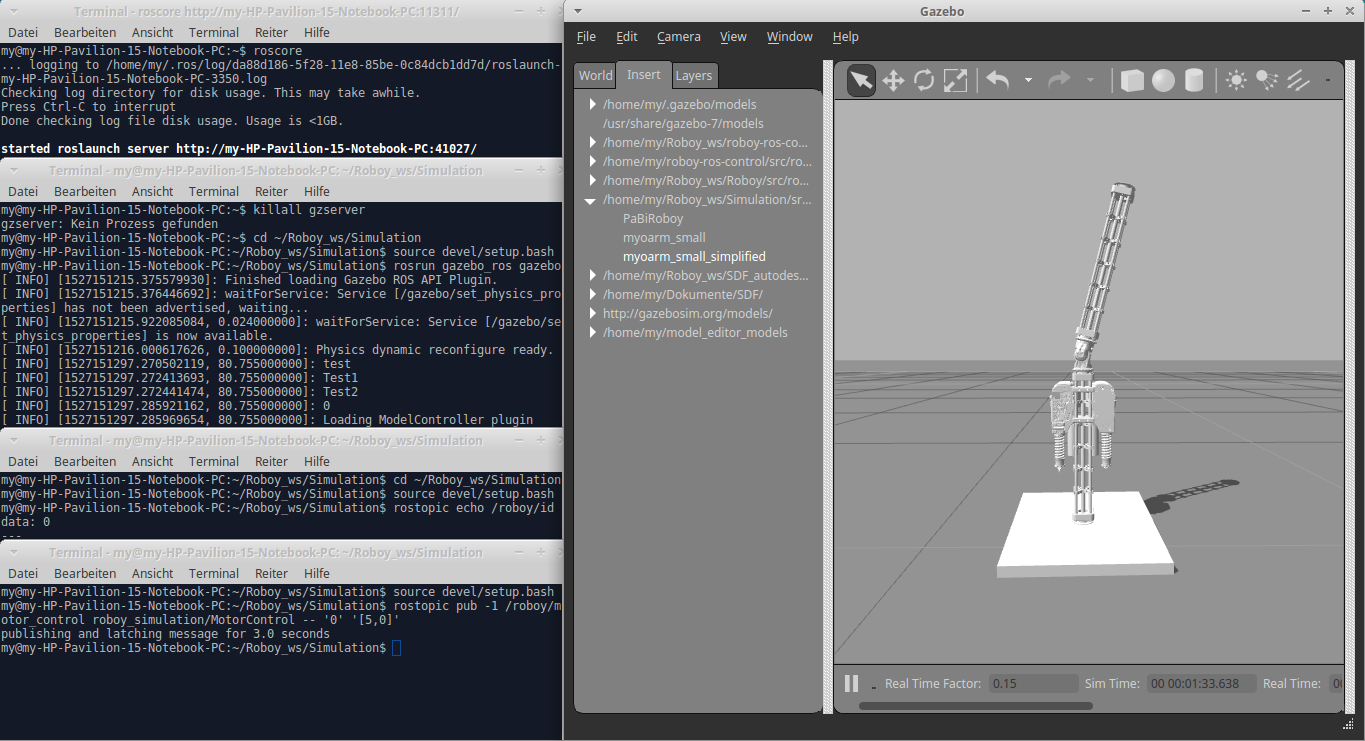
\includegraphics[width=0.9\textwidth] {figures/2.png}
   %\label{fig:PP_L_COM1_A}
 %}
 \caption{Example of Roboy simulation}
 \label{fig:Roboy}
\end{figure}

The option \codew{‘-1’} sends the command only once. Otherwise, the forces are sent constantly. The Roboy id, here ‘0’, is usually 0 for the first robot and then it increments with each new robot. The size of the voltage array, here 2 with ‘[10,0]’ , depends on the number of joints or muscles. This number can be determined by checking the plug-in tag in the SDFormat file of the robot model.% When using the command line, it is helpful to use tab complete, e.g.\ type \codew{rostopic pub -1 /roboy/} and click on the tab key twice. This lists all possible options or - if only one options exists -automatically completes a part of the command.

If the real time factor is low when using the MyoMuscle plug-in in Gazebo, there can be a large lag between sending the command and the reaction of the robot. This can possibly be avoided by using models with \_simplified in their name. However, depending on the PC that is used, the real time factor can be very low even with small models. This is unfeasible and undesired for research and development, as real-time simulations are required for realistic experiments.

Furthermore, some joints  are only able to handle limited forces. It is necessary to not go above the limits or else the robot model can end up flying around. This problem has yet to be solved, as this behavior prevents efficient operation. In these cases, the robot has to be loaded again or Gazebo even  has to be restarted. Even with smaller forces, the robot model sometimes appears to be unstable, with the robot model shaking.

Some other improvements have to be made, such as optimization of step size or calculation of tendon length after the limit of the forces has been reached\cite{BA}.

The problems mentioned above highlight the shortcomings of the current simulation. Therefore, the simulation and control of tendon-driven robots has yet to be improved.